% GENERATED by `bench paper` — do not edit.
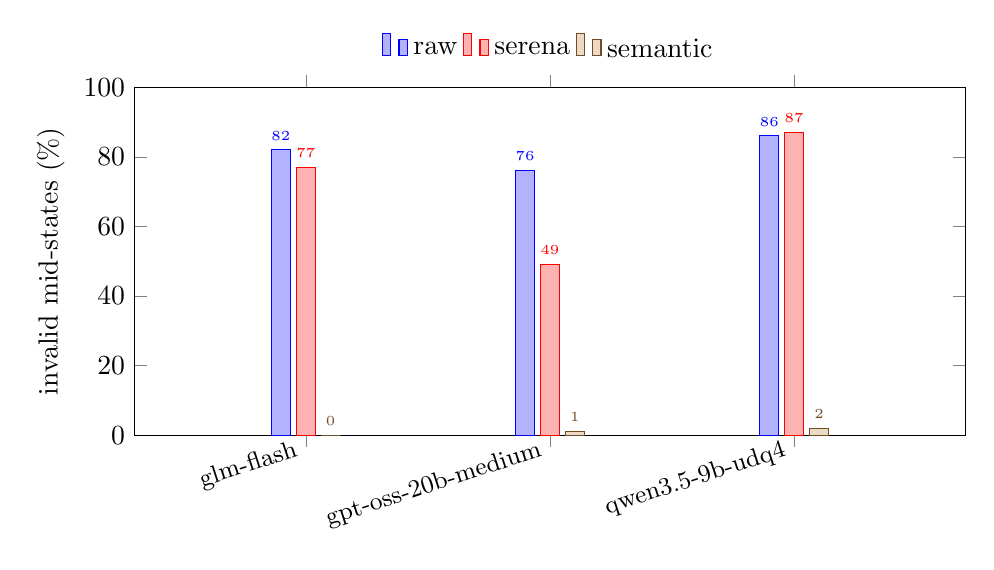
\begin{tikzpicture}
\begin{axis}[
  ybar, bar width=7pt, width=\linewidth, height=6cm,
  ymin=0, ymax=100, ylabel={invalid mid-states (\%)},
  symbolic x coords={glm-flash,gpt-oss-20b-medium,qwen3.5-9b-udq4},
  xtick=data, x tick label style={rotate=18,anchor=east,font=\small},
  legend style={at={(0.5,1.04)},anchor=south,legend columns=-1,draw=none},
  enlarge x limits=0.35, nodes near coords,
  every node near coord/.append style={font=\tiny,/pgf/number format/precision=0,/pgf/number format/fixed},
]
\addplot coordinates {(glm-flash,82) (gpt-oss-20b-medium,76) (qwen3.5-9b-udq4,86)};
\addplot coordinates {(glm-flash,77) (gpt-oss-20b-medium,49) (qwen3.5-9b-udq4,87)};
\addplot coordinates {(glm-flash,0) (gpt-oss-20b-medium,1) (qwen3.5-9b-udq4,2)};
\legend{raw, serena, semantic}
\end{axis}
\end{tikzpicture}
